\section{Weighted Arithmetic Mean}

\Cref{fig:weighted} displays a scatter plot illustrating the relationship between validation accuracy and the weighted arithmetic mean. Every data point displayed within the graph corresponds to a unique architecture evaluated during the experiment. A dotted red line represents the best-fit linear regression line through the data points. Additionally, the graph includes Spearman's rank correlation coefficient in the title, which measures the monotonic relationship between the validation accuracy and the weighted arithmetic mean. 

\begin{figure}[h!]
  \centering
  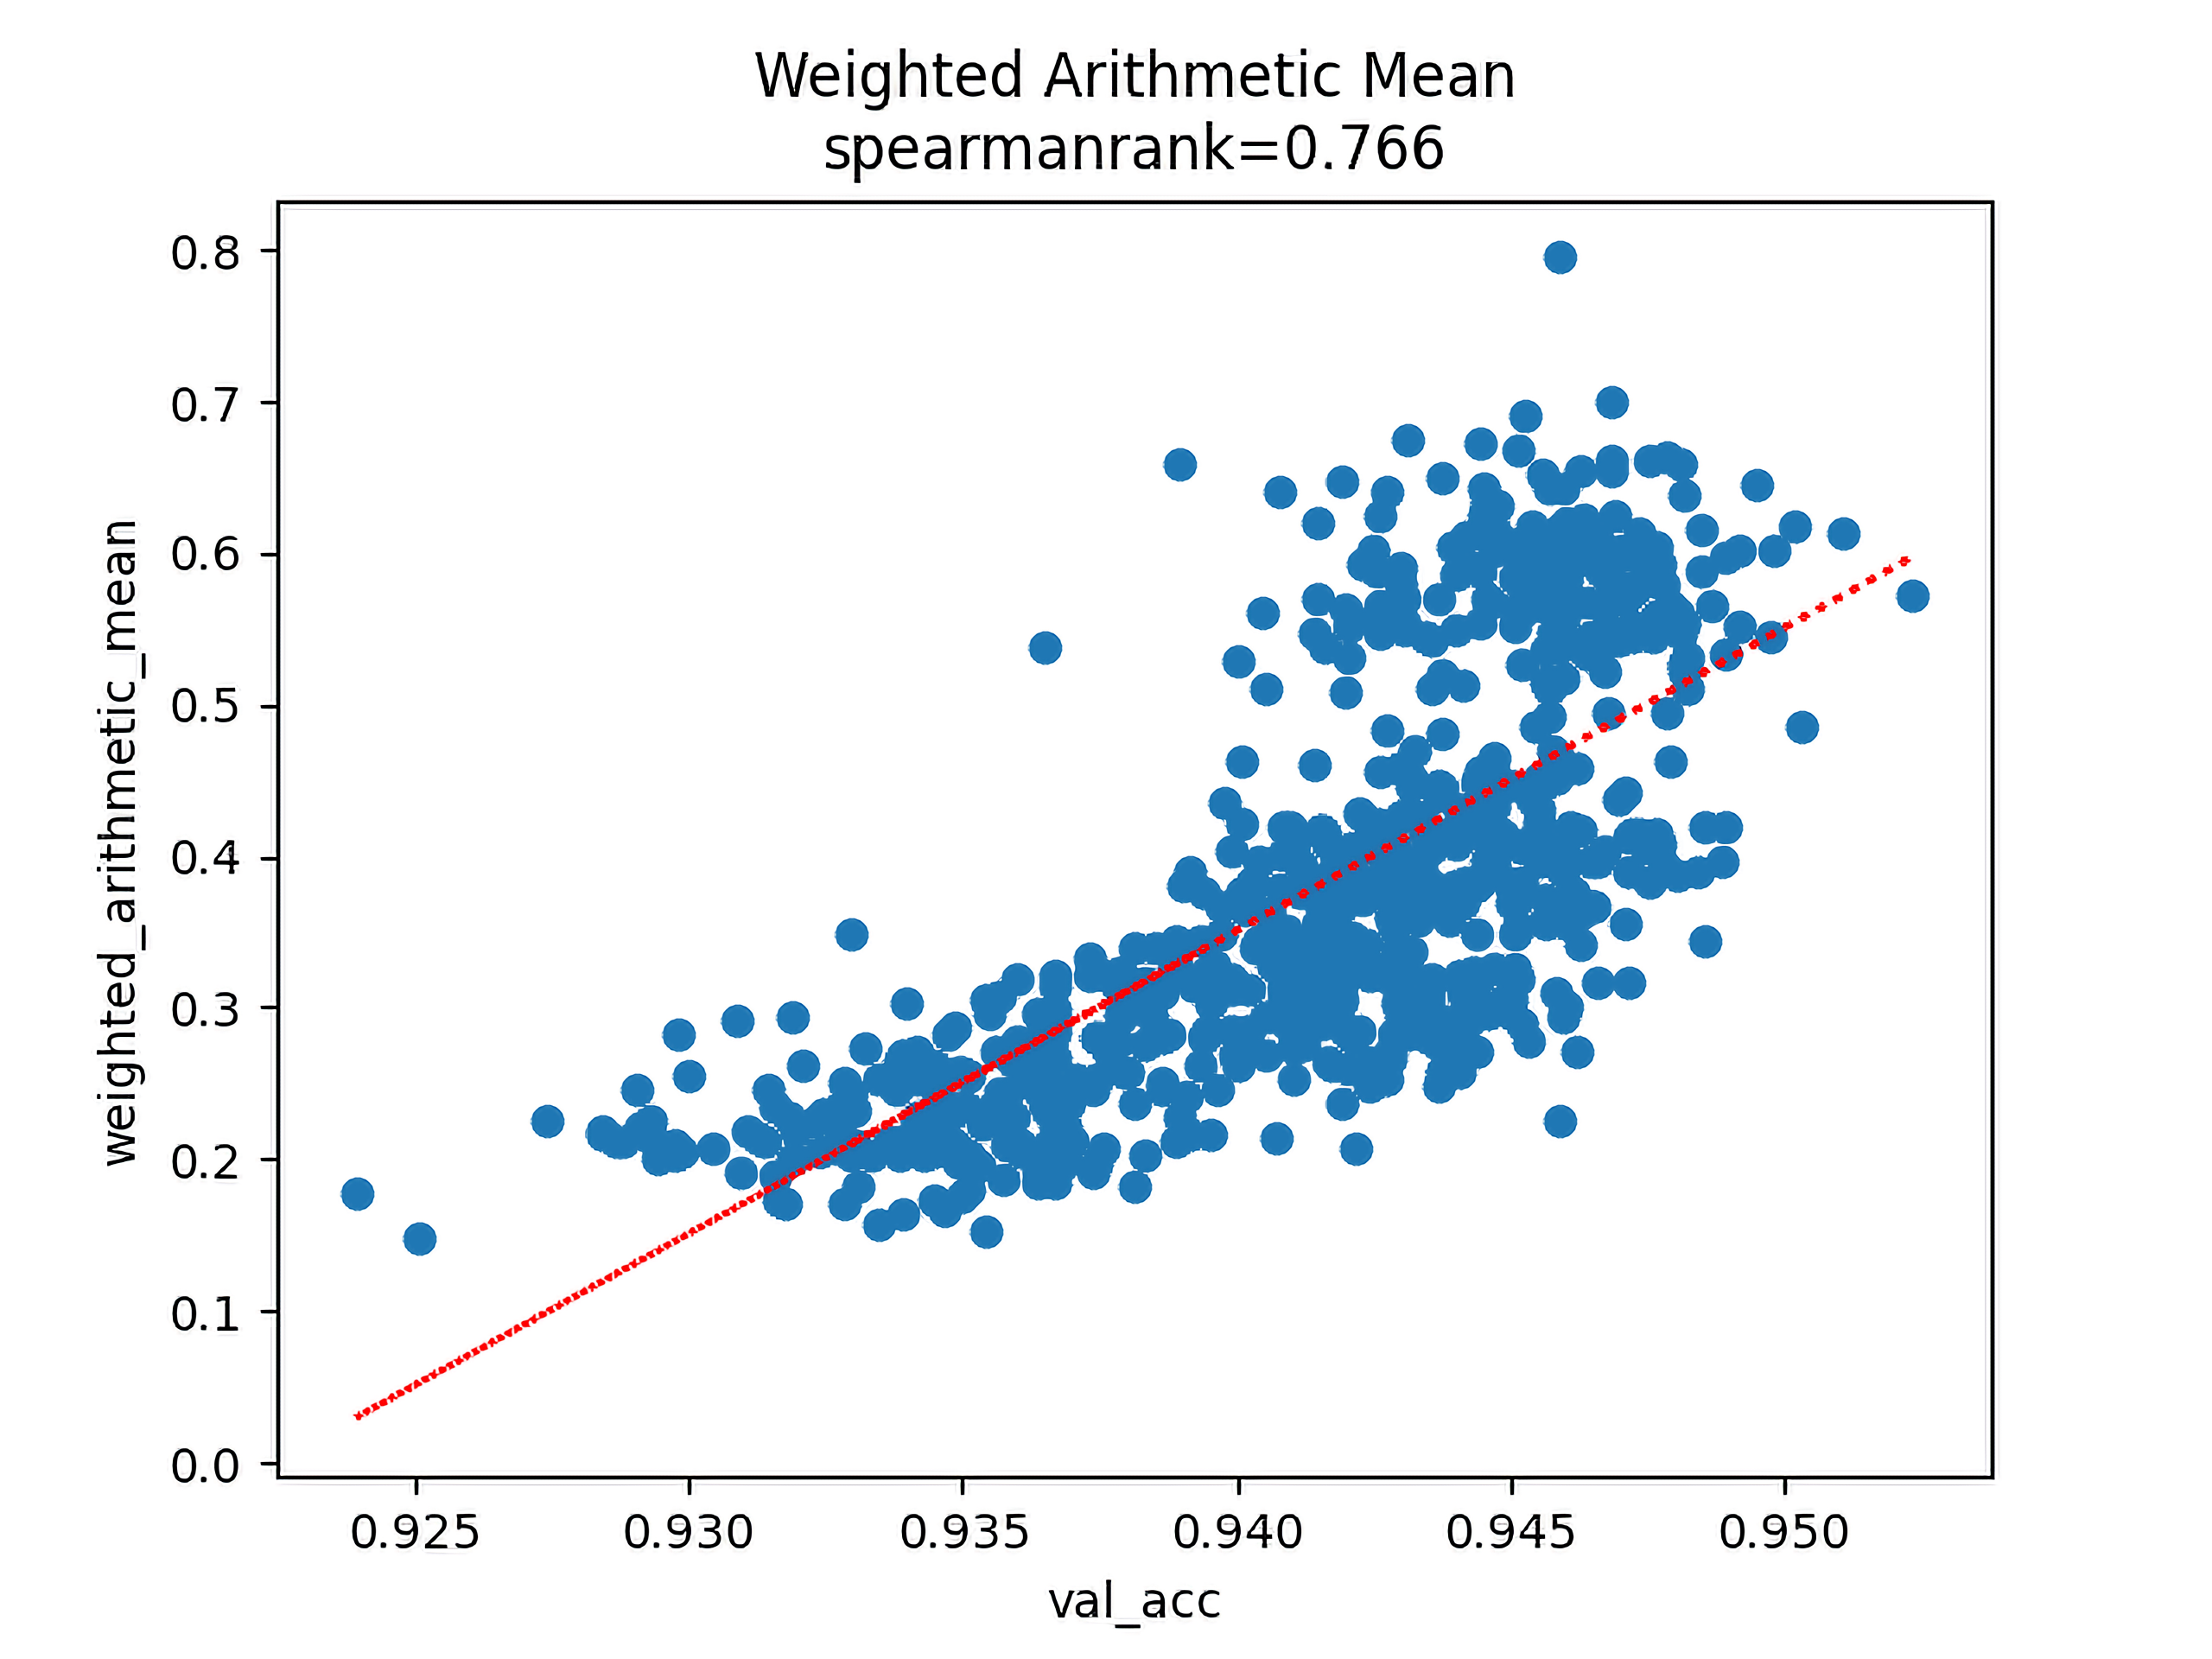
\includegraphics[width=0.9\columnwidth]{figures/weighted_average_upscaled.png}
  \caption{Weighted Arithmetic Mean}
  \label{fig:weighted}
\end{figure}